\onecolumn

\section{Analysis on Natural and Synthetic Data Distributions}
\label{app:data_distribution_analysis}

\begin{figure}[h]
    \centering
    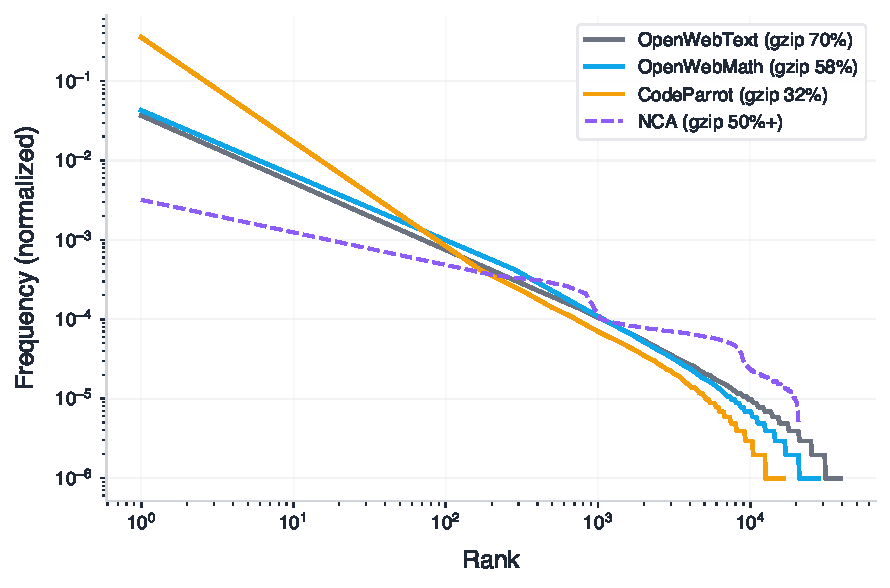
\includegraphics[width=0.5\linewidth]{figures/token_distribution.pdf}
    \caption{\textbf{NCA data exhibits a similar Zipfian or power-law structure to natural language.} We compare the relative token frequency distribution for each of the natural language corpora and NCA data. Natural language from different domains has different average complexity as measured by gzip compressibility (see legend).}
    \label{fig:token-distributions}
\end{figure}

\begin{figure}[t]
    \centering
    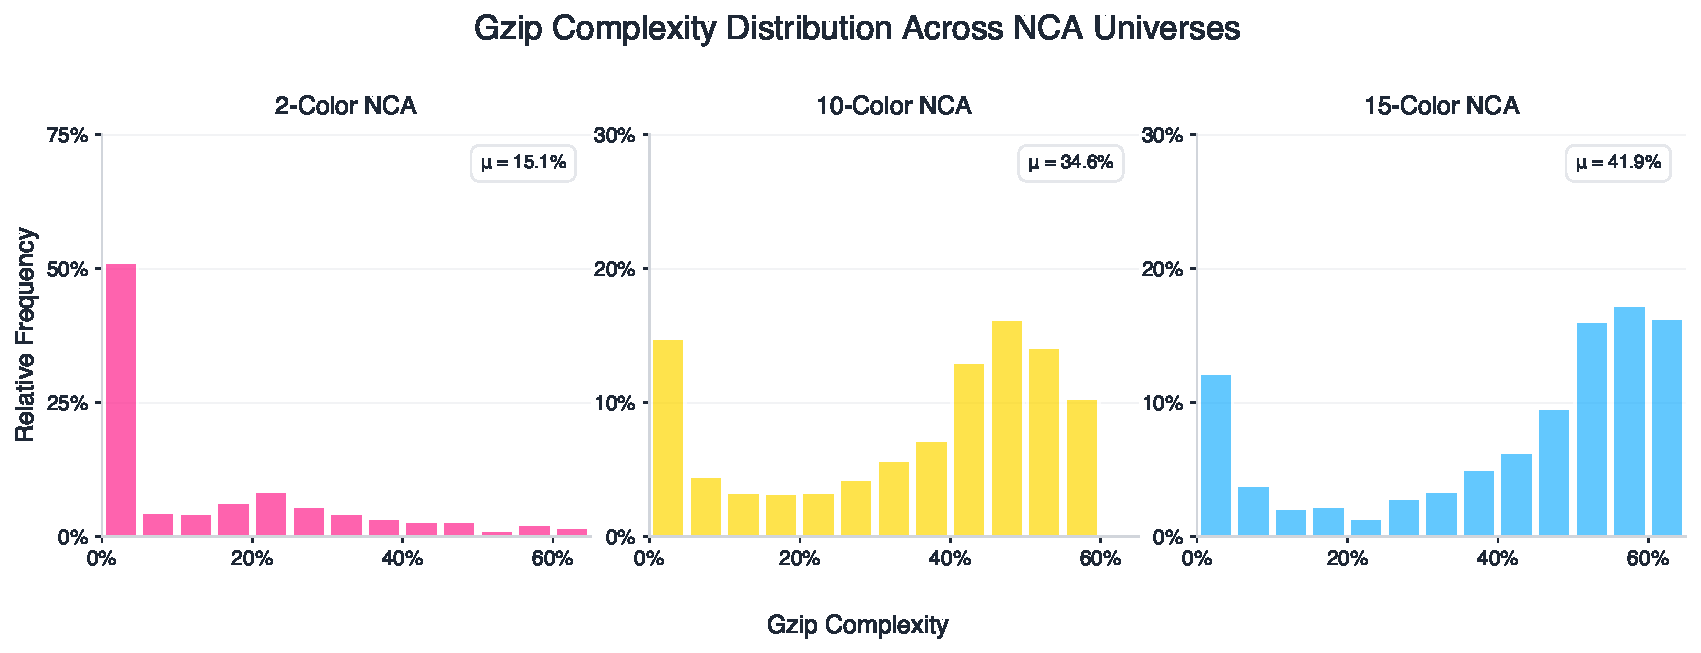
\includegraphics[width=\linewidth]{figures/gzip_complexity_distribution.pdf}
    \caption{Different NCA alphabet sizes, $n=2,10,15$ naturally yield different complexity distributions of the data. Increasing $n$ inherently increases the complexity of the data.}
    \label{fig:nca_gzip}
\end{figure}

In this section, we examine the distributions of natural-language and NCA-generated synthetic data with respect to two primary high-order heuristics: (1) token frequency distribution and (2) gzip compressibility.
\subsection{NCA data exhibits similar token distributions to natural language}
To compare the token frequency across different data distributions, we sample and tokenize random text sequences from the natural language datasets (OpenWebText, OpenWebMath, and CodeParrot) and NCA generated data ($n=15$). Figure~\ref{fig:token-distributions} shows the distribution of relative token frequencies. Data generated from the NCAs follows a heavy-tailed, Zipfian token distribution that is structured similarly to natural language. Another interesting observation is that natural language depending on the domain varies quite drastically from 32\% in code and 60-70\% in math and web text.

\subsection{Increasing the vocabulary size $n$ leads to more complex generated trajectories}
Figure~\ref{fig:nca_gzip} compares the distribution of gzip complexity across trajectories generated by randomly sampled NCAs across different alphabet sizes $n=2,10,15$. As $n$ increases, the distribution skews towards less compressible, more complex data. This implies that with higher $n$, the universe of rules expands and naturally the dynamics become more complex.

% \dl{Thought here: This could imply (1) that GZIP isn't as good of a metric for distinguishability at high $n$ or (2) high $n$ have more complex sequences and rules.}
\section{Detailed Pre-pre-training and Pre-training Setup}
\label{app:experimental-setup}

Table~\ref{tab:hyperparams} summarizes the hyperparameters used for both pre-pre-training on NCA data and subsequent pretraining on natural language datasets. We sweep various batch sizes (32 to 512), learning rates ($1\times10^{-3}$ to $1\times10^{-5}$), and weight decays ($1\times10^{-4}$ to $1\times 10^{-6}$). To ensure reproducibility, we train our pipeline on 4 randomness seeds for each main pipeline (NCA Pre-pre-training, Scratch, and C4 Pre-pre-training) and at least 2 seeds for each ablation run.

\begin{table}[h]
\centering
\small
\setlength{\tabcolsep}{6pt}
\renewcommand{\arraystretch}{1.15}
\begin{tabular}{lcc}
\toprule
\textbf{Hyperparameter} & \textbf{Pre-pre-training} & \textbf{Pre-training} \\
\midrule
Effective batch size & 16 & 512 \\
Sequence length & 1024 tokens & 1024 tokens \\
Learning rate & $1 \times 10^{-4}$ & $5 \times 10^{-4}$ (Math/Text), $2\times 10^{-4}$ (Code) \\
LR schedule & Cosine w/ warmup & Cosine w/ warmup \\
Warmup steps (\% total) & 10\% & 10\% \\
Weight decay & None & $1 \times 10^{-4}$ \\
Gradient clipping & None & 1.0 \\
\bottomrule
\end{tabular}
\caption{Hyperparameters for pre-pre-training and pre-training experiments.}
\label{tab:hyperparams}
\end{table}
\section{Detailed Fine-Tuning Setup}
\label{app:instruction-ft-setup}
For GSM8K and HumanEval, we evaluate on all tasks provided by the benchmarks. For BigBench-Lite, given the quantity and imbalance of samples and tasks, we randomly sample at most 300 tasks for each major category of english language problem where there are at least 100 examples available for training.

For GSM8K and BigBench-Lite, we fine-tune the OpenWebMath and OpenWebText pre-trained models on the respective training sets. For GSM8K, we train for 10 epochs using a learning rate of 1e-5 to enable the models to follow the question answering format for evaluation. For GSM8k, we also fine-tune on the Chain-of-Thought reasoning trace provided by the dataset. For BigBench-Lite, we train for a single epoch at a learning rate of 5e-6 to enable models to follow the answer format. Across both we sweep hyperparameters including learning and choose the best performing models for comparison for each baseline and NCA pre-trained model. For HumanEval, we do not fine-tune the models since it is a code completion task. For reproducibility, we train 4 seeds for each model and baseline and report the averages across runs.

We evaluate the models' performances across different Pass@$k$ with $k$ varying from 1, 8, 16, and 32. For Big-Bench, because of the multiple-choice nature of some tasks, we opt to demonstrate up to 4 passes. We use the unbiased estimator from \citet{chen2021evaluating}, computing the metric from 64 total decodings per run. For evaluation, we sampled with a temperature of $0.4$ and top-p of $0.95$ across GSM8k, HumanEval, and BigBench. We evaluated with higher temperatures and use $0.4$ temperature as higher temperatures led to overall worse and highly variable performance. We use 4 training pipeline seeds per task for each baseline and NCA pre-pretrained models and 5 decoding seeds per pipeline seed.


\section{NCA Pre-Pre-Training is more token efficient than natural language}
\label{app:token-efficiency}
In this section, we compare convergence speed across pipelines by computing a different the token efficiency metric used in  \citet{hu2025circuitschomskyprepretrainingformal}. Token efficiency gain is defined as: $\text{Token Efficiency Gain} = 1 - \frac{T_{\text{PPT}}^{\text{NCA}} + T_{\text{PT}}^{\text{NCA}}}{T_{\text{PPT}}^{\text{base}} + T_{\text{PT}}^{\text{base}}}$. Where $T_{\text{PPT}}$ represents the number of pre-pre-training tokens and $T_{\text{PT}}$ represents the number of pre-training tokens to achieve the scratch model's final loss. Note that $T_{\text{PPT}}^{\text{base}} = 0$ for the no pre-pre-training baseline.

On average, NCA pre-pre-trained models exhibit token efficiency gains of 31\% on OpenWebText, 27\% on OpenWebMath, and 49\% on CodeParrot to reach equivalent performance to the scratch baseline.